\documentclass[a4paper,12pt]{article}
\usepackage[utf8]{inputenc}
\usepackage{amsfonts,amstext}
\usepackage{amsmath,amssymb}
\usepackage{amsthm}
% \usepackage{german}
\usepackage[ngerman]{babel}
\usepackage{fullpage}
\usepackage[a4paper,margin=3cm]{geometry}
\usepackage{hyperref}
\usepackage{listings}
\usepackage[usenames,dvipsnames]{xcolor}
% \usepackage[noend]{algpseudocode}
% \usepackage{algorithm}
\usepackage{fancyhdr}
\usepackage{lastpage}
\usepackage{graphicx}
\usepackage{float}
\usepackage{bookmark}
\usepackage[parfill]{parskip} % https://tex.stackexchange.com/questions/74170/have-new-line-between-paragraphs-no-indentation#74173



% https://www.overleaf.com/learn/latex/Theorems_and_proofs
% https://www.overleaf.com/learn/latex/Theorems_and_proofs#Reference_guide
\theoremstyle{definition}
\newtheorem*{example}{Beispiel}
\newtheorem{definition}{Definition}[section]

\theoremstyle{plain}
\newtheorem{theorem}{Satz}[section]
\newtheorem{lemma}[definition]{Lemma}

\theoremstyle{remark}
\newtheorem*{remark}{Bemerkung}
\newtheorem*{notation}{Notation}
\newtheorem*{question}{Frage}


% Defining \lsem and \rsem without using MnSymbol
\newcommand{\lsem}{\mathrm{[}\kern-.14em\mathrm{[}}
\newcommand{\rsem}{\mathrm{]}\kern-.14em\mathrm{]}}
\newcommand{\zb}{z.\,B.\;}
\renewcommand{\dh}{d.\,h.\;}
\newcommand{\floor}[1]{\left\lfloor{#1}\right\rfloor}
\newcommand{\ceil}[1]{\left\lceil{#1}\right\rceil}
\newcommand{\half}[1]{\frac{#1}{2}}
\newcommand{\sem}[1]{S\lsem#1\rsem}
\newcommand{\Bsem}[1]{\mathcal{B}\lsem#1\rsem}
\newcommand{\Asem}[1]{\mathcal{A}\lsem#1\rsem}
\newcommand{\Nsem}[1]{\mathcal{N}\lsem#1\rsem}
\newcommand{\Ssem}[1]{\mathcal{S}\lsem#1\rsem}
\newcommand{\strans}[3]{\langle #1, #2 \rangle \to #3}

\newcommand{\figref}[1]{Abbildung~\ref{#1}}
\newcommand{\secref}[1]{Abschnitt~\ref{#1}}
\newcommand{\defref}[1]{Definition~\ref{#1}}
\newcommand{\defrefshort}[1]{\text{D.}~\ref{#1}}  % for math mode

\DeclareMathOperator{\bits}{\{0,1\}}
\DeclareMathOperator{\AExp}{AExp}
\DeclareMathOperator{\BExp}{BExp}
\DeclareMathOperator{\SExp}{SExp}
\DeclareMathOperator{\Stm}{Stm}
\DeclareMathOperator{\Num}{Num}
\DeclareMathOperator{\Var}{Var}
\DeclareMathOperator{\State}{State}
\DeclareMathOperator{\A}{\mathcal{A}}
\DeclareMathOperator{\B}{\mathcal{B}}
\DeclareMathOperator{\N}{\mathcal{N}}
\DeclareMathOperator{\FV}{FV}
\DeclareMathOperator{\true}{w}
\DeclareMathOperator{\false}{f}

\renewcommand{\labelenumi}{(\alph{enumi})}


\definecolor{codegreen}{rgb}{0,0.6,0}
\definecolor{codegray}{rgb}{0.5,0.5,0.5}
\definecolor{codepurple}{rgb}{0.58,0,0.82}
\definecolor{backcolor}{rgb}{0.95,0.95,0.95}

\lstdefinestyle{mystyle}{
    backgroundcolor=\color{backcolor},
    commentstyle=\color{codegreen},
    keywordstyle=\color{magenta},
    numberstyle=\tiny\color{codegray},
    stringstyle=\color{codepurple},
    basicstyle=\ttfamily\small,
    breakatwhitespace=false,
    breaklines=true,
    captionpos=b,
    keepspaces=true,
    numbers=left,
    numbersep=6pt,
    showspaces=false,
    showstringspaces=false,
    showtabs=false,
    tabsize=2
}
\lstset{style=mystyle}
% \lstset{language=C}


\setlength{\headheight}{14.5pt}
\setlength{\headsep}{16pt}
\pagestyle{fancy}
\fancyhf{}
\renewcommand{\headrulewidth}{2pt}
\renewcommand{\footrulewidth}{1pt}
\lhead{\leftmark}
% \rhead{\rightmark}
\cfoot{Seite \thepage \,von \pageref{LastPage}}



\begin{document}

% \title{
%     Semantik von Programmiersprachen \\[6pt]
%     \large Vorlesung SoSe 2022 \\
%     Wolfgang Mulzer
% }
% \author{Jim Neuendorf}
% \maketitle
% \begin{abstract}
%     \noindent Diese Vorlesung vermittelt Techniken zur Formalisierung der Semantik (Be"-deu"-tungs"-inhalte) von Programmiersprachen. Zunächst werden unter"-schied"-liche Forma"-li"-sie"-rungs"-ansätze (die operationelle, denotationelle und axio"-ma"-ti"-sche Semantik) vorgestellt und diskutiert. Anschließend wird die mathe"-ma"-ti"-sche Theorie der semantischen Bereiche behandelt, die bei der deno"-tatio"-nel"-len Methode, Anwendung findet. Danach wird schrittweise eine umfassende, impe"-rative Programmiersprache entwickelt und die Semantik der einzelnen Sprach"-ele"-mente denotationell spezifiziert. Dabei wird die Fortsetzungstechnik (con"-tinua"-tion sem) systematisch erklärt und verwendet. Schließlich wird auf die Anwendung dieser Techniken eingegangen, insbesondere im Rahmen des Com"-piler"-baus und als Grundlage zur Entwicklung funktionaler Programmier"-spra"-chen.
% \end{abstract}
\title{
    Semantik von Programmiersprachen \\[6pt]
    \large Vorlesung SoSe 2022 \\
    Wolfgang Mulzer
}
\author{Jim Neuendorf}
\maketitle
\begin{abstract}
    \noindent Diese Vorlesung vermittelt Techniken zur Formalisierung der Semantik (Be"-deu"-tungs"-inhalte) von Programmiersprachen. Zunächst werden unter"-schied"-liche Forma"-li"-sie"-rungs"-ansätze (die operationelle, denotationelle und axio"-ma"-ti"-sche Semantik) vorgestellt und diskutiert. Anschließend wird die mathe"-ma"-ti"-sche Theorie der semantischen Bereiche behandelt, die bei der deno"-tatio"-nel"-len Methode, Anwendung findet. Danach wird schrittweise eine umfassende, impe"-rative Programmiersprache entwickelt und die Semantik der einzelnen Sprach"-ele"-mente denotationell spezifiziert. Dabei wird die Fortsetzungstechnik (con"-tinua"-tion sem) systematisch erklärt und verwendet. Schließlich wird auf die Anwendung dieser Techniken eingegangen, insbesondere im Rahmen des Com"-piler"-baus und als Grundlage zur Entwicklung funktionaler Programmier"-spra"-chen.
\end{abstract}


\newpage
\tableofcontents


% \newpage
% \hfill 29.04.

% \section{Semantik}


% Ziel: Finde eine mathematische Methode, um einem Programm eine \emph{Bedeutung} zuzuordnen.

% Motivation:
% \begin{itemize}
%     \item Verifikation:
%         \begin{itemize}
%             \item Erfüllt mein Programm die Spezifikation (tut es das, was es soll)?
%             \item Setzt der Übersetzer/Interpretierer die Spezifikation der Sprache korrekt um?
%         \end{itemize}
%      \item Programmumformung
%         \begin{itemize}
%             \item Haben zwei unterschiedliche Programme die gleiche Bedeutung?
%             \item Optimierung
%         \end{itemize}
%     \item Programmanalyse
%         \begin{itemize}
%             \item Ist das Programm ``sicher'' (secure vs. safe)?
%             \item Ist das Programm ``effizient''?
%         \end{itemize}
% \end{itemize}

% \begin{definition}[Programmierparadigma]
%     Programmierparadigma: \zb deklarativ (``Was?'') (funktional vs. logisch), imperativ (``Wie?''). In verschiedenen Paradigmen haben (potenziell) Programme verschiedene Bedeutungen.
% \end{definition}

% Wir konzentrieren uns auf \emph{imperative} Programmierung.

% \begin{question}
%     Was ist die ``mathematische Bedeutung'' eines imperativen Programms?
% \end{question}

% \begin{question}[folgend]
%     Was ist ein imperatives Programm?
% \end{question}



% \begin{lstlisting}[language=Python, caption=Imperatives Programm]
% x = 1
% y = x + 2
% x = y + 5
% for ...
% \end{lstlisting}
% % => Es gibt einen Zustand (alles, was im Speicher steht). Diesen ändert man mit Zuweisung


% \begin{lstlisting}[language=Haskell, caption=Funktionales Programm]
% foo :: Int -> Int
% foo 0 = 1
% foo x = x + 1
% foo 3
% \end{lstlisting}
% % => kein Zustand, sondern es gibt einen Ausdruck, der ausgewertet wird

% Das zentrale Konzept der imperativen Programmierung ist der \emph{Zustand} (state). Der Zustand ist der Inhalt aller Speicherzellen und Register, die Position des Programm"-zählers und der Zustand der Eingabe-/Ausgabe-Geräte.

% Ein imperatives Programm ist eine Folge von \emph{Anweisungen} (statement / instruction). Diese haben \emph{Wirkungen} (effects), welche den Zustand verändern (selbst \texttt{nop} ändert den Programmzähler und somit den Zustand). Darüber hinasu gibt es Neben"-wir"-kungen bzw. Seiteneffekte (side effects). Es gibt unterschiedliche Arten von Anwei"-sungen:
% \begin{itemize}
%     \item Zuweisungen (direkte Änderung des Zustandes)
%     \item Kontrollfluss (Änderung des Programmzählers: Verzweigungen, Schleifen, Funk"-tions"-aufrufe bzw. Sprünge)
%     \item Eingabe / Ausgabe
% \end{itemize}
\hfill 29.04.

\section{Semantik}


Ziel: Finde eine mathematische Methode, um einem Programm eine \emph{Bedeutung} zuzuordnen.

Motivation:
\begin{itemize}
    \item Verifikation:
        \begin{itemize}
            \item Erfüllt mein Programm die Spezifikation (tut es das, was es soll)?
            \item Setzt der Übersetzer/Interpretierer die Spezifikation der Sprache korrekt um?
        \end{itemize}
     \item Programmumformung
        \begin{itemize}
            \item Haben zwei unterschiedliche Programme die gleiche Bedeutung?
            \item Optimierung
        \end{itemize}
    \item Programmanalyse
        \begin{itemize}
            \item Ist das Programm ``sicher'' (secure vs. safe)?
            \item Ist das Programm ``effizient''?
        \end{itemize}
\end{itemize}

\begin{definition}[Programmierparadigma]
    Programmierparadigma: \zb deklarativ (``Was?'') (funktional vs. logisch), imperativ (``Wie?''). In verschiedenen Paradigmen haben (potenziell) Programme verschiedene Bedeutungen.
\end{definition}

Wir konzentrieren uns auf \emph{imperative} Programmierung.

\begin{question}
    Was ist die ``mathematische Bedeutung'' eines imperativen Programms?
\end{question}

\begin{question}[folgend]
    Was ist ein imperatives Programm?
\end{question}



\begin{lstlisting}[language=Python, caption=Imperatives Programm]
x = 1
y = x + 2
x = y + 5
for ...
\end{lstlisting}
% => Es gibt einen Zustand (alles, was im Speicher steht). Diesen ändert man mit Zuweisung


\begin{lstlisting}[language=Haskell, caption=Funktionales Programm]
foo :: Int -> Int
foo 0 = 1
foo x = x + 1
foo 3
\end{lstlisting}
% => kein Zustand, sondern es gibt einen Ausdruck, der ausgewertet wird

Das zentrale Konzept der imperativen Programmierung ist der \emph{Zustand} (state). Der Zustand ist der Inhalt aller Speicherzellen und Register, die Position des Programm"-zählers und der Zustand der Eingabe-/Ausgabe-Geräte.

Ein imperatives Programm ist eine Folge von \emph{Anweisungen} (statement / instruction). Diese haben \emph{Wirkungen} (effects), welche den Zustand verändern (selbst \texttt{nop} ändert den Programmzähler und somit den Zustand). Darüber hinasu gibt es Neben"-wir"-kungen bzw. Seiteneffekte (side effects). Es gibt unterschiedliche Arten von Anwei"-sungen:
\begin{itemize}
    \item Zuweisungen (direkte Änderung des Zustandes)
    \item Kontrollfluss (Änderung des Programmzählers: Verzweigungen, Schleifen, Funk"-tions"-aufrufe bzw. Sprünge)
    \item Eingabe / Ausgabe
\end{itemize}


%%%%%%%%%%%%%%%%%%%%%%%%%%%%%%%%%%%%%%%%%%%%%%%%%%%%%%%%%%%%%%
\newpage
\section{Mathematische Formalisierung}

\begin{definition}[Zustand]
    Es gibt eine abzählbar unendliche Menge von Variablen $V = \{ x_1, x_2, \dots, y, z, \dots \}$ (Speicher ist begrenzt aber beliebig groß). Der Zustand ist eine (partielle) Funktion $$\sigma: V \to \mathbb{Z} \cup \{ \bot, true, false \}$$ ($\bot$ bedeutet undefiniert, \dh eine Speicherzelle hat noch keinen Wert und die Funk"-tion gibt nichts aus).

    Die Teile des Zustandes ``Eingabe / Ausgabe'' ignorieren wir erst einmal, \dh die initiale Eingabe ist implizit durch den Wert der Variablen am Anfang. Der Programm"-zähler wird an anderer Stelle thematisiert.
\end{definition}

\begin{remark}
    Diese Definition dient als Bespiel, \dh in anderen Szenarion mit anderen Variables außer Ganzzahlen und Boolesche Wert kann eine andere Definition sinnvoller sein.
\end{remark}

\begin{definition}[Imperatives Programm]
    Ein imperatives Programm ist eine Funktion auf der Menge alles Zustände. Jedem Startzustand wird ein Endzustand zugeordnet (wir ignorieren E/A).
\end{definition}

\begin{notation}
    Sei $\Pi \in \Sigma^*$ ein gültiges Programm (eine Zeichenkette). Wir bezeichnen mit
    $$\sem{\Pi} \in [State \to State]$$
    ($S$ ist die semantische Funktion) die Funktion, welche durch $\Pi$ definiert wird.
\end{notation}


\subsection{\texttt{while}-Sprache} \label{section:while}

\begin{definition}
    Wir verwenden in dieser Vorlesung eine einfache, turing-vollständige, imperative Programmiersprache als durchgängiges Beispiel namens \texttt{while}\emph{-Sprache}, die durch folgende kontextfreie Grammatik gegeben ist:
\end{definition}
\vspace*{-2em}
\begin{align*}
    A & \to \texttt{Zahl | Var | $A + A$ | $A * A$ | $A - A$} \\
    B & \to \texttt{true | false | $A = A$ | $A \leq A$ | $\neg B$ | $B \wedge B$} \\
    S & \to \texttt{Var := A | skip | S; S | if B then S else S | while B do S}
\end{align*}
\begin{remark}
    Es gibt die syntaktischen Kategorien ``arithmetischer Ausdruck'' ($A$), ``Boolescher Ausdruck'' ($B$) und ``Statement'' ($S$, Anweisung).
\end{remark}

\begin{example}
    \begin{align*}
        \Pi & = \texttt{x = z + 1;} \\
        \Ssem{\texttt{x = z + 1;}}(\underbrace{[x \mapsto 5, z \mapsto -4, a \mapsto 2]}_{\text{Startzustand}}) & = \underbrace{[x \mapsto -3, z \mapsto 4, a \mapsto 2]}_{\text{Endzustand}} \\
        \Ssem{\texttt{x = z + 3;}}([x \mapsto 10, z \mapsto 12]) & = [x \mapsto 10, z \mapsto 12]
    \end{align*}
\end{example}

\fbox{Für diese Veranstaltung stellen wir uns die Frage: Wie komme ich von $\Pi$ zu $\sem{\Pi}$?}


Dafür gibt es drei Ansätze:
\begin{enumerate}
    \item axiomatische Semantik
    \item operationelle Semantik
    \item denotationelle Semantik
\end{enumerate}


\subsection{Axiomatische Semantik}

Wir verzichten auf die vollständige Spezifikation von $\sem{\cdot}$. Stattdessen arbeiten wir mit \emph{Zusicherungen} (Assertions), welche wesentliche Aspekte des Zustands zu einem gegebenen Zeitpunkt widerspiegeln.

Wir definieren ein logisches System, das Beziehungen zwischen Zuständen aufstellt (Vorbedingungen, Nachebdingungen). Das System muss $\sem{\cdot}$ verträglich sein.

Die Details sind Thema einer anderen Vorlesungen, \zb Hoare-Kalkül.

\begin{example}
    $$\underbrace{\{ x = n \wedge y = m \}}_{\text{Vorbedingung}} \quad \texttt{z := x; x := y; y := z} \quad \underbrace{\{ x = m \wedge y = n \}}_{\text{Nachbedingung}}$$
\end{example}



\subsection{Operationelle Semantik}

Definiere $\sem{\Pi}$ durch schrittweise Simulation der Ausführung von $\Pi$ (ein Interpretierer in mathematischer Form / Abstraktion).

Genauer gesagt bedeutet das: Wir definieren ein \emph{Transitionssystem}
\begin{align*}
    \langle \Pi, s \rangle & \Rightarrow \langle \Pi', s' \rangle \\
    \langle \Pi, s \rangle & \Rightarrow s'
\end{align*}
das die Ausführung von $\Pi$ auf Zustand $s$ darstellt.

\begin{example}
    \begin{align*}
        & \langle \texttt{'z = x; x = y; y = z;'}, [x \mapsto 2, y \mapsto 3, z \mapsto 6] \rangle \\
        \leadsto \; & \langle \texttt{'x = y; y = z;'}, [x \mapsto 2, y \mapsto 3, z \mapsto 2] \rangle \quad\quad \text{(1. Befehl ausgeführt)} \\
        \leadsto \; & \langle \texttt{'y = z;'}, [x \mapsto 3, y \mapsto 3, z \mapsto 2] \rangle \\
        \leadsto \; & [x \mapsto 3, y \mapsto 2, z \mapsto 2] \quad\quad \text{(Endzustand)}
    \end{align*}
\end{example}



%%%%%%%%%%%%%%%%%%%%%%%%%%%%%%%%%%%%%%%%%%%%%%%%%%%%%%%%%%%%%%%%%%%%%
\newpage
\hfill 06.05.
%%%%%%%%%%%%%%%%%%%%%%%%%%%%%%%%%%%%%%%%%%%%%%%%%%%%%%%%%%%%%%%%%%%%%


\subsection{Denotationelle Semantik}

Definiere $\sem{\Pi}$ direkt als mathematisch Funktion anhand der Syntax von $\Pi$, \zb
\begin{align*}
    \Ssem{\texttt{z := x; x := y; y := z}} & = \Ssem{\texttt{y := z}} \circ \Ssem{\texttt{x := y}} \circ \Ssem{\texttt{z := x}}
\end{align*}

Es wird also \zb die sequenzielle Ausführung von Anweisungen als Funktionskomposition übersetzt.

\begin{remark}[Problem]
    Wie kann man beispielsweise Schleifen darstellen (insbesondere \texttt{while})? Ein möglicher Ansatz sind Grenzwerte, aber das geht tiefer in die Analysis.

    Bei der operationellen Semantik wird die Schleife durch das Transitionssystem realisiert.
\end{remark}



%%%%%%%%%%%%%%%%%%%%%%%%%%%%%%%%%%%%%%%%%%%%%%%%%%%%%%%%%%%%%%
\newpage
\section{Operationelle Semantik}

Das Folgende bezieht sich auf die \texttt{while}-Sprache (siehe \secref{section:while}).

\begin{definition}
    $\AExp, \BExp, \Stm$: Mengen aller gültigen Ableitungen aus A, B, S als Syntaxbaum. Der Ausdruck \texttt{5+7-2*8} lässt sich aus $A$ ableiten. Der entsprechende Syntaxbaum (siehe \figref{fig:syntaxbaum}) ist dann Teil von $\AExp$.
    $$a \in \AExp$$
    Mengen wie $\AExp$ bezeichnen wir als \textbf{syntaktische Kategorien}.

    \textbf{Zahl} ist eine ganze Zahl aus $\mathbb{Z}$. Die zugehörige syntaktische Kategorie $\Num$. Num ist die Menge aller Zeichenkette, die ganze Zahlen darstellen.
    \begin{align*}
        \texttt{1234} & \in \Num \\
        1234 & \in \mathbb{Z}
    \end{align*}
    Beachte, dass eigentlich der Syntaxbaum von \texttt{1234} gemeint ist

    $\Var$ sind Variablen, die nach Belieben vorhanden sind. Es sind abzählbar unendlich viele.
\end{definition}

% https://dreampuf.github.io/GraphvizOnline/
% digraph G {
%     ordering="out";
%     mult[label="*"];
%     minus[label="-"];
%     plus[label="+"];
%     zahl1[label="Zahl"]; zahl2[label="Zahl"]; zahl3[label="Zahl"]; zahl4[label="Zahl"];
%     minus -> plus -> zahl1 -> 5;
%              plus -> zahl2 -> 7;
%     minus -> mult -> zahl3 -> 2;
%              mult -> zahl4 -> 8;
% }
\begin{figure}[H]
    \centering
    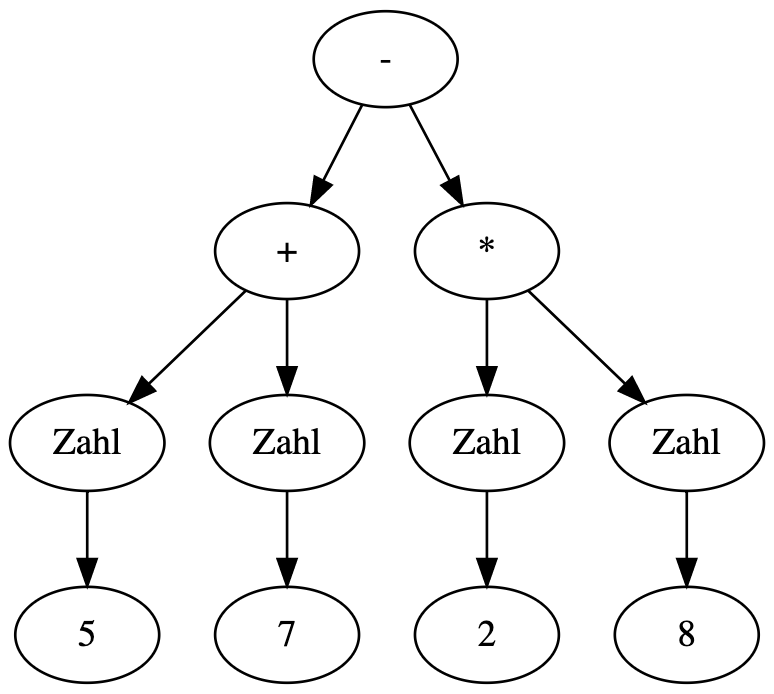
\includegraphics[width=.4\textwidth]{syntaxbaum.png}
    \caption{\texttt{5+7-2*8} $\in \AExp$ als verkürzt dargestellter Syntaxbaum}
    \label{fig:syntaxbaum}
\end{figure}

\begin{remark}
    Unterbäume können auch Elemente einer anderen Kategorie sein.
    % B -> (A < A) \in BExp
    % Unterbaum A \in AExp
\end{remark}

\begin{example}
    Division mit Rest
    \begin{itemize}
        \item Eingabe: $a, b > 0$
        \item Ausgabe: $m ,r \geq 0$, $r < b$, $a = m \cdot b + r$
    \end{itemize}
\end{example}

\begin{lstlisting}[language=C, caption=Division mit Rest]
m := 0;
while b <= a do (
    m := m + 1;
    a := a - b
)
r := a
\end{lstlisting}

Die \emph{Semantik} in \texttt{while} wird gegeben durch eine \emph{semantische Funktion}, eine für jede \emph{syntaktische Kategorie}.

Sei $State = \{ \sigma \,\vert\, \sigma: \Var \to \mathbb{Z} \}$, \zb
\begin{align*}
    \mathcal{N} : \Num & \to \mathbb{Z} \\
    \mathcal{N}\lsem\texttt{-123}\rsem & = -123
\end{align*}

\begin{align*}
    \A: \underbrace{\AExp}_{\text{``Compiler''}} & \to \underbrace{(\State \to \mathbb{Z})}_{\text{``Interpreter''}} \\
    \A\lsem\texttt{x+x*5}\rsem & = (\sigma \mapsto 6 \cdot \sigma(x)) \quad (\text{da }\texttt{x+x*5} = \texttt{6*x})
\end{align*}

\begin{align*}
    \B : \BExp \to (\State \to \{ w, f \}) \\
    \B\lsem\texttt{x<=10}\rsem = \bigg( \sigma \mapsto \begin{cases}
        w & \sigma(x) \leq 10 \\
        f & \sigma(x) > 10
    \end{cases} \bigg)
\end{align*}

$$S: \Stm \to (\State + \State)$$

\textbf{Jetzt:} Definition von $\A$ durch Induktion über die Struktur des Syntaxbaums. Die Definition von $\N$ und $\B$ ist eine Übung.

\textbf{Später:} Definition von $S$.


\subsection{Semantik arithmetischer Ausdrücke}

\begin{definition}[Induktive Definition von $\A$] \label{def:Asem}
    Sei $n \in \Num, x \in \Var, \sigma \in \State$ und $a_1, a_2 \in \AExp$. Wir definieren:
    \begin{enumerate}
        \item[(i)] $\A\lsem n \rsem(\sigma) = \N\lsem n \rsem$ \quad\quad (konstante Funktion)
        \item[(ii)] $\A\lsem x \rsem(\sigma) = \sigma(x)$ \quad\quad\quad alternativ: $\A\lsem n \rsem = (\sigma \mapsto \sigma(n))$
        \item[(iii)] $\A\lsem a_1 + a_2 \rsem(\sigma) = \A\lsem a_1 \rsem(\sigma) + \A\lsem a_2 \rsem(\sigma)$ \\[4pt]
        \emph{Bemerkung.} In anderen Sprachen könnte der Aufruf des ersten Summanden Seiteneffekte haben, \dh ggf. muss man an dieser Stelle aufpassen. In diesem Fall würde der potentenziell veränderte Zustand mit zurückgegeben werden.
        \item[(iv)] Analog für Subtraktion
        \item[(v)] Analog für Multiplikation
    \end{enumerate}
\end{definition}

\begin{remark}
    Für die Definition von semantischen Funktionen fordern wir \textbf{Zusammengesetztheit}, \dh in der induktiven Definition darf nur auf Bestandteile des Ausdrucks/Syntaxbaums zugegriffen werden.
\end{remark}

\begin{example}
    Führe Negation ein : $\A \to \dots | -A$.

    Erlaubt ist $\A\lsem -a_1 \rsem(\sigma) = 0 - \A\lsem a_1 \rsem(\sigma)$ aber nicht $\A\lsem -a_1 \rsem(\sigma) = \A\lsem 0 - a_1 \rsem(\sigma)$, da der Ausdruck hier um eine Null erweitert wurde.
\end{example}



%%%%%%%%%%%%%%%%%%%%%%%%%%%%%%%%%%%%%%%%%%%%%%%%%%%%%%%%%%%%%%%%%%%%%
\newpage
\hfill 13.05.
%%%%%%%%%%%%%%%%%%%%%%%%%%%%%%%%%%%%%%%%%%%%%%%%%%%%%%%%%%%%%%%%%%%%%

\begin{theorem}
    $\A$ besitzt die folgenden Eigenschaften:
    \begin{enumerate}
        \item für alle $a \in \AExp$, für alle $\sigma \in \State$ existiert genau eine Zahl $n \in \mathbb{Z}$, sodass $\A\lsem a \rsem (\sigma) = n$. (Voraussetzung: $\sigma$ ist eine totale Funktion.)
        \item $\A$ ist eine totale Funktion.
    \end{enumerate}
\end{theorem}

\begin{proof}[Beweis]
    Skizze:
    \begin{enumerate}
        \item[(b)] folgt aus (a)
        \item[(a)] wird bewiesen durch strukturelle Induktion nach $a$.
    \end{enumerate}
\end{proof}

\par\bigskip
\textbf{Nächste Schritte:}
\begin{enumerate}
    \item[(i)] Der Wert eines Ausdrucks hängt \emph{nur} von den Variables ab, die in ihm vorkommen. (\secref{section:freeVars})
    \item[(ii)] Was passiert in einem arithmetischen Ausdruck, wenn wir eine Variable durch einen Ausdruck ersetzen ($\leadsto$ \emph{Substitution})? (\secref{section:substitution})
\end{enumerate}



% FREIE VARIABLEN %%%%%%%%%%%%%%%%%%%%%%%%%%%%%%%%%%%%%%%%%%%%%%%%%%%%%%%%%%%%%%%%%%%%%%%%%%%
\subsection{Freie Variablen} \label{section:freeVars}

\begin{definition}[Freie Variablen]
    Sei $a \in \AExp$. $\FV(a)$ (``freie Variablen'') ist die Menge aller Variablen, die in $a$ vorkommen. Formal ist das induktiv definiert:
    \begin{enumerate}
        \item $\FV(n) = \emptyset$ \quad\quad\quad (falls $a = n$ (Zahl))
        \item $\FV(x) = \{ x \}$ \quad\quad (falls $a = x$ (Variable))
        \item $\FV(a_1 \;\square\; a_2) = \FV(a_1) \cup \FV(a_2)$ \quad\quad für $\square \in \{ +, -, * \}$
    \end{enumerate}

    Gebundene Variable betrachten wir im Kontekt der \texttt{while}-Sprache nicht. in anderen Sprachen können aber lokale Variablen \zb als solche betrachtet werden.
\end{definition}

\begin{lemma}
    Sei $a \in \AExp$, sei $\sigma, \sigma' \in \State$, sodass $\sigma(x) = \sigma'(x)$ für alle $x \ in\FV(a)$ gilt.

    Dann gilt: $$\A\lsem a \rsem(\sigma) = \A\lsem a \rsem(\sigma')$$
\end{lemma}
\begin{proof}[Beweis]
    Durch strukturelle Induktion nach $a$.

    \emph{Induktionsanfang:}
    \begin{enumerate}
        \item $a = n$, $n$ Zahl
            \begin{align*}
                \A\lsem a \rsem(\sigma) & = \A\lsem n \rsem(\sigma) \\
                & \overset{\defrefshort{def:Asem}(i)}{=} \N\lsem n \rsem \\
                \\
                \A\lsem a \rsem(\sigma') & = \A\lsem n \rsem(\sigma') \\
                & = \N\lsem n \rsem
            \end{align*}

        \item $a = x$, $x$ Variable
            \begin{align*}
                \A\lsem a \rsem(\sigma) & = \A\lsem x \rsem(\sigma) \\
                & \overset{\defrefshort{def:Asem}(ii)}{=} \sigma(x) \\
                \\
                \A\lsem a \rsem(\sigma') & = \A\lsem x \rsem(\sigma') \\
                & = \sigma'(x) \\
                \\
                \FV(a) & = \FV(x) = \{ x \}
            \end{align*}
            Nach Annahme ist $\sigma(x) = \sigma'(x)$, da $x \in \FV(a)$. Daher folgt
            $$\A\lsem a \rsem(\sigma) = \A\lsem a \rsem(\sigma')$$
    \end{enumerate}

    \emph{Induktionsschritt:}

    $a = a_1 \;\square\; a_2$ mit $\square \in \{ +, -, * \}$

    \begin{align*}
        \A\lsem a \rsem(\sigma) & = \A\lsem a_1 \;\square\; a_2 \rsem(\sigma) \\
        & = \A\lsem a_1 \rsem(\sigma) \;\square\; \A\lsem a_2 \rsem(\sigma) \\
        \\
        \A\lsem a \rsem(\sigma') & = \A\lsem a_1 \;\square\; a_2 \rsem(\sigma') \\
        & = \A\lsem a_1 \rsem(\sigma') \;\square\; \A\lsem a_2 \rsem(\sigma') \\
        \\
        \FV(a) & = \FV(a_1 \;\square\; a_2) \\
        & = \FV(a_1) \cup \FV(a_2)
    \end{align*}
    Insbesondere gilt, dass $\FV(a_1) \subseteq \FV(a)$ und $\FV(a_2) \subseteq \FV(a)$. Daher folgt:

    Da nach Annahme $\sigma(x) = \sigma(x')$ für alle $x \in \FV(a)$, gilt
    $$\sigma(x) = \sigma'(x) \text{ für alle } x \in \FV(a_1)$$
    und
    $$\sigma(x) = \sigma'(x) \text{ für alle } x \in \FV(a_2)$$

    Also gelten nach Induktionsvoraussetzung
    $$\A\lsem a_1 \rsem(\sigma) = \A\lsem a_1 \rsem(\sigma') \wedge \A\lsem a_2 \rsem(\sigma) = \A\lsem a_2 \rsem(\sigma')$$

    Daher folgt:
    $$\A\lsem a_1 \rsem(\sigma) \;\square\; \A\lsem a_2 \rsem(\sigma) = \A\lsem a_1 \rsem(\sigma') \;\square\; \A\lsem a_2 \rsem(\sigma')$$
\end{proof}



% SUBSTITUTION %%%%%%%%%%%%%%%%%%%%%%%%%%%%%%%%%%%%%%%%%%%%%%%%%%%%%%%%%%%%%%%%%%%%%%%%%%%%%%%%
\subsection{Substitution} \label{section:substitution}

\begin{definition}[Substitution für Ausdrücke] \label{def:substitutionExp}
    Seien $a, a_0 \in \AExp, \, y \in \Var$. Wir definieren $a[y \mapsto a_0]$ als den arithmetischen Ausdruck, in dem jedes Vorkommen von $y$ in $a$ durch $a_0$ ersetzt wird.

    Formal:
    \begin{enumerate}
        \item[(i)] $n[y \mapsto a_0] = n$
        \item[(ii)] $x[y \mapsto a_0] = \begin{cases} a_0 & \text{falls } x = y \\ x & \text{sonst} \end{cases}$
        \item[(iii)] $(a_1 \;\square\; a_2)[y \mapsto a_0] = a_1[y \mapsto a_0] \;\square\; a_2[y \mapsto a_0]$ \quad\quad für $\square \in \{ +, -, * \}$
    \end{enumerate}
\end{definition}

\begin{example}
    \begin{align*}
        a & = \texttt{x + y*2 - z(x + y)} \\
        \texttt{y} & \mapsto \texttt{4*t + 5} \\
        \\
        a[\texttt{y} \mapsto \texttt{4*t + 5}] & = \texttt{x + (4*t + 5)*2 - z(x + (4*t + 5))}
    \end{align*}
    Es werden die Blätter am Syntaxbaum ersetzt, woraus implizit die Präzedenz klar ist (wodurch die obigen Klammern entstehen).

    Ersetzungen dürfen die zu ersetzende Variable enthalten. Da nur einmal ersetzt wird, ist das in Ordnung.
\end{example}

\begin{definition}[Substitution für Zustände] \label{def:substitutionState}
    Sei $\sigma \in \State, \, x \in \Var, \, n \in \mathbb{Z}$. Dann ist $\sigma[x \mapsto n] \in \State$ der Zustand, der wie folgt definiert ist:
    \begin{align*}
        \sigma[x \mapsto n](z) = \begin{cases}
            n & \text{falls } z = x \\
            \sigma(z) & \text{sonst}
        \end{cases}
    \end{align*}
\end{definition}

\begin{lemma}
    Sei $a, a_0 \in \AExp, \, y \in \Var, \, \sigma \in \State$. Dann gilt:
    \begin{align*}
        \A\lsem a[y \mapsto a_0] \rsem(\sigma) & = \A\lsem a \rsem \Big( \sigma\big[y \mapsto \A\lsem a_0 \rsem(\sigma)\big] \Big)
    \end{align*}
\end{lemma}

Das Lemma setzt Semantik und Syntax in Verbindung: Wir können syntaktisch Variable durch Teilausdrücke ersetzen und das ist äquivalent dazu, erst den Teilausdruck auszuwerten und mit diesen Wert im Zustand den ursprünglichen Ausdruck auszuwerten.

\begin{example}
    \begin{align*}
    a & = x + y \\
    a_0 & = x * y \\
    \sigma: & \; [x \mapsto 2; y \mapsto 10] \\
    \\
    (x + (x * y))[x \mapsto 2; y \mapsto 10] \quad & \square\; (x + y)[x \mapsto 2; y \mapsto 20] \\
    2 + (2 * 10) \quad & \square\; 2 + 20 \\
    22 \quad & = 22
\end{align*}
\end{example}


\begin{proof}[Beweis]
    Durch strukturelle Induktion nach $a$ (nicht $a_0$!).

    \emph{Induktionsanfang:}
    \begin{enumerate}
        \item $a = n$, $n$ Zahl
            \begin{align*}
                \A\lsem a[y \mapsto a_0] \rsem(\sigma) & = \A\lsem n[y \mapsto a_0] \rsem(\sigma) \\
                & \overset{\defrefshort{def:substitutionExp}(i)}{=} \A\lsem n \rsem(\sigma) \\
                & = n \\
                \\
                \A\lsem n \rsem(\sigma[y \mapsto \A\lsem a_0 \rsem(\sigma)]) & = n \quad\quad \text{(rechte Seite)}
            \end{align*}

        \item $a = x$, $x$ Variable
            \begin{align*}
                \A\lsem x[y \mapsto a_0] \rsem(\sigma) & \overset{\defrefshort{def:substitutionExp}(iii)}{=} \begin{cases}
                    \A\lsem a_0 \rsem(\sigma) & \text{falls } x = y \\
                    \A\lsem x \rsem(\sigma) = \sigma(x) & \text{sonst}
                \end{cases} \\
                \\
                \A\lsem x \rsem(\sigma[y \mapsto \A\lsem a_0 \rsem(\sigma)]) & \overset{\defrefshort{def:substitutionState}}{=} (\sigma[y \mapsto \A\lsem a_0 \rsem(\sigma)])(x) \quad\quad \text{(rechte Seite)} \\
                & = \begin{cases}
                    \A\lsem a_0 \rsem(\sigma) & \text{falls } x = y \\
                    \sigma(x) & \text{sonst}
                \end{cases}
            \end{align*}
    \end{enumerate}

    \emph{Induktionsschritt:} Straight forward.
\end{proof}



%%%%%%%%%%%%%%%%%%%%%%%%%%%%%%%%%%%%%%%%%%%%%%%%%%%%%%%%%%%%%%%%%%%%%
\newpage
\hfill 20.05.
%%%%%%%%%%%%%%%%%%%%%%%%%%%%%%%%%%%%%%%%%%%%%%%%%%%%%%%%%%%%%%%%%%%%%
\subsection{Definition von \texorpdfstring{$\mathcal{S}\lsem \cdot \rsem$}{S[.]}}

$\Asem{\cdot}$ und $\Bsem{\cdot}$ \emph{benutzen} den Zustand $\sigma$ während die Semantik von Anweisungen den Zustand \emph{verändern} soll.

``Big Step'' operationelle Semantik (\emph{natürliche Semantik}).

Idee: Definiere $\Ssem{\cdot}$ mithilfe einer Zustandsüberführungerelation.

\begin{definition}
    Sei $s \in \SExp$ eine Anweisungsfolge und seien $\sigma, \sigma' \in \State$ Zustände. Die Zustandsüberführungsrelation
    $$\strans{S}{\sigma}{\sigma'}$$
    spezifiziert die Beziehung zwischen Startzustand $\sigma$ und dem Endzustand $\sigma'$ gemäß der Anweisungsfolge $S$.
\end{definition}

\begin{remark}[Bedeutung]
    Die Ausführung von $S$ auf Startzustand $\sigma$ terminiert mit Endzustand $\sigma'$.
\end{remark}

\par\medskip
\begin{notation}
    Wir definieren die Zustandsübergangsrelation mithilfe von Schlussregeln. Eine solche Schlussregel besitzt die folgende Form:
    $$\frac{\text{Voraussetzung}}{\text{Folgerung}} \leadsto \frac{\strans{S_1}{\sigma_1}{\sigma_1'}, \strans{S_2}{\sigma_2}{\sigma_2'}, \,\dots\, , \strans{S_n}{\sigma_n}{\sigma_n'}}{\strans{S}{\sigma}{\sigma'}}$$
    (ggf. mit zusätzlichen Bedingungen) wobei $S_1, \dots, S_n$ Bestandteile von $S$ sind.

    Gibt es keine Voraussetzung, nennen wir die Schlussregel ein \emph{Axiom}.
\end{notation}



% SCHLUSSREGELN %%%%%%%%%%%%%%%%%%%%%%%%%%%%%%%%%%%%%%%%%%%%%%%%%%%%%%%%%%%%%%%%%%%%%%%%%%%%%%%
\subsubsection{Schlussregeln für die natürliche Semantik von \texttt{while}}

Im Folgenden schreiben wir x$_{\text{ns}}$ um anzuzeigen, dass es sich um die natürliche Semantik handelt.

\begin{enumerate}
    \item Zuweisung $[\text{zuw}_{\text{ns}}]$ (Axiom)
    $$\frac{}{\strans{x \texttt{ := } a}{\sigma}{\sigma[x \mapsto \Asem{a}(\sigma)]}}$$

    \item Skip $[\text{skip}_{\text{ns}}]$ (Axiom)
    $$\frac{}{\strans{\texttt{skip}}{\sigma}{\sigma}}$$

    \item Hintereinanderausführung $[\text{seq}_{\text{ns}}]$
    $$\frac{\strans{S_1}{\sigma}{\sigma'}, \strans{S_2}{\sigma'}{\sigma''}}{\strans{S_1 \texttt{;} S_2}{\sigma}{\sigma''}}$$
    Dabei können $S_1$ und $S_2$ zusammengesetzte Anweisungen sein.

    \item Verzweigung $[\text{if}_{\text{ns}}^{\true}]$
    $$\frac{\strans{S_1}{\sigma}{\sigma'}}{\strans{\texttt{if } b \texttt{ then } S_1 \texttt{ else } S_2}{\sigma}{\sigma'}}$$
    falls $\Bsem{b}(\sigma) = \true$. Dabei muss $S_2$ nicht terminieren.

    \item Verzweigung $[\text{if}_{\text{ns}}^{\false}]$
    $$\frac{\langle S_2, \sigma \rangle \to \sigma'}{\langle \texttt{if } b \texttt{ then } S_1 \texttt{ else } S_2, \sigma \rangle \to \sigma'}$$
    falls $\Bsem{b}(\sigma) = \false$. Dabei muss $S_1$ nicht terminieren.

    \item Schleife $[\text{while}_{\text{ns}}^{\true}]$
    $$\frac{\langle S, \sigma \rangle \to \sigma', \langle \texttt{while } b \texttt{ do } S, \sigma' \rangle \to \sigma''}{\langle \texttt{while } b \texttt{ do } S, \sigma \rangle \to \sigma''}$$
    falls $\Bsem{b}(\sigma) = \true$. Im Allgemeinen kann es sein, dass die Schleife nicht terminiert. Deshalb müssen wir diesen Fall in der Definition der semantischen Funktion beachten. Das bedeutet, diese Relation ist nicht total.

    \item Schleife $[\text{while}_{\text{ns}}^{\false}]$
    $$\frac{\text{ }}{\langle \texttt{while } b \texttt{ do } S, \sigma \rangle \to \sigma}$$
    falls $\Bsem{b}(\sigma) = \false$.
\end{enumerate}

\par\bigskip
\par\bigskip
Wie ist die Zustandsüberführungsfunktion überhaupt definiert?

\begin{definition}
    Sei $S \in \SExp$ ein Programm und seien $\sigma, \sigma' \in \State$. Dann gilt
    $$\langle S, \sigma \rangle \to \sigma'$$ gdw. ein \emph{endlicher Ableitungsbaum} dafür existiert.

    Der Ableitungsbaum entsteht durch wiederholte Anwendung der Schlussregeln . Die Wurzel ist ist $\langle S, \sigma \rangle \to \sigma'$, die Blätter sind Axiome, die Knoten entsprechen  korrekte Anwendung der Schlussregeln.
\end{definition}

\begin{example}
    Sei $\sigma \in \State$ mit $\sigma(x) = 1$ und $\sigma(y) = 5$.

    Behauptung: $\langle (z := z; x := y); y := z, \sigma \rangle \to \sigma[z \mapsto 1][x \mapsto 5][y \mapsto 1]$

    Nun müssen wir den endlichen Ableitungsbaum erzeugen.


    \begin{enumerate}
        \item $[\text{seq}_{ns}]$
            $$\frac{\langle z := x; x ;= y, \sigma \rangle \to \sigma', \langle y := z, \sigma' \rangle \to \sigma[z \mapsto 1][x \mapsto 5][y \mapsto 1]}{\langle \underbrace{(z := z; x := y)}_{s_1}; \underbrace{y := z}_{S_2}, \sigma \rangle \to \sigma[z \mapsto 1][x \mapsto 5][y \mapsto 1]}$$

            Welches $\sigma'$ brauchen wir? $\leadsto \sigma[z \mapsto 1][x \mapsto 5]$. Somit erhalten wir
            $$\frac{\langle z := x; x := y, \sigma \rangle \to \sigma[z \mapsto 1][x \mapsto 5], \langle y := z, \sigma[z \mapsto 1][x \mapsto 5] \rangle \to \sigma[z \mapsto 1][x \mapsto 5][y \mapsto 1]}{\langle \underbrace{(z := z; x := y)}_{S_1}; \underbrace{y := z}_{S_2}, \sigma \rangle \to \sigma[z \mapsto 1][x \mapsto 5][y \mapsto 1]}$$

        \item $[\text{zuw}_{ns}]$ für den rechten Teil
            $$\frac{\Asem{z}(\sigma[z \mapsto 1][x \mapsto 5]) \overset{?}{=} 1}{\langle y := z, \sigma[z \mapsto 1][x \mapsto 5] \rangle \to \sigma[z \mapsto 1][x \mapsto 5][y \mapsto 1]}$$

            $$\Asem{z}(\sigma[z \mapsto 1][x \mapsto 5]) \overset{Def}{=} \sigma[z \mapsto 1][x \mapsto 5](z) \overset{Def}{=} 1$$

        \item $[\text{seq}_{ns}]$
            $$\frac{\langle z := x, \sigma \rangle \to \sigma[z \mapsto 1], \langle x := y, \sigma[z \mapsto 1] \rangle \to \sigma[z \mapsto 1][x \mapsto 5]}{\langle z := x; x ;= y, \sigma \rangle \to \sigma[z \mapsto 1][x \mapsto 5]}$$

            Ab hier analog zum rechten Teil (mit zwei Mal $[\text{zuw}_{ns}]$).
    \end{enumerate}
\end{example}

\par\bigskip
\begin{remark}[Rechtseindeutigkeit / Determiniertheit]
    Es ist noch nicht klar, dass ``$\to$'' \emph{rechtseindeutig} ist. D.\,h. möglicherweise existiert ein Programm $S$, ein Startzustand $\sigma$ und Zustände $\sigma_1 \neq \sigma_2 \in \State$, sodass sowohl
    $$\langle S, \sigma \rangle \to \sigma_1 \text{ als auch } \langle S, \sigma \rangle \to \sigma_2$$
    gilt. Daher muss die Rechtseindeutigkeit bzw. \emph{Determiniertheit} bewiesen werden!
\end{remark}

\par\medskip
\begin{remark}[Ableitungsbaum]
    Der Ableitungsbaum ist statisch. D.\,h. man kann nicht erkennen, in welcher Reihenfolge die Schlussregeln angewendet werden.
\end{remark}







\end{document}
